\RequirePackage{xcolor} % to use xcolor in jhep3
%\documentclass[11pt,note]{HONGBOANU}                                                                                                                                
\documentclass[11pt,assignment]{HONGBOANU}
%\documentclass[11pt]{HONGBOANU}


%\usepackage{amsmath}
\usepackage{graphicx}
%\usepackage{amssymb}
%\usepackage{latexsym}
%\usepackage{dcolumn}% Align table columns on decimal point
%\usepackage{bm}% bold math
%\usepackage{epsfig,multicol,bbm}
\usepackage{listings}% to insert codes in tex
%\usepackage[framed,numbered,autolinebreaks,useliterate]{mcode} %inline code enviroment
\usepackage{multirow} %multi-line in tabular
\usepackage{float} % fix the position of table
%\usepackage{color}
%\usepackage{xcolor}
%\usepackage{epstopdf}
%\usepackage[T1]{fontenc}
%\usepackage[latin9]{inputenc}
%\usepackage{units}
%\usepackage{esint}
\usepackage{fancyhdr}
\pagestyle{fancy}
%\usepackage{marginnote}
%\usepackage[top=Bcm, bottom=Hcm, outer=Ccm, inner=Acm, heightrounded, marginparwidth=Ecm, marginparsep=Dcm]{geometry}


%\setlength{\textwidth}{17cm} %
\setlength{\textheight}{25cm} %
%\setlength{\topmargin}{0.5cm} %
%\setlength{\oddsidemargin}{2cm} %
\setlength{\footskip}{1cm}
%multi-line in tabular
\newcommand{\tabincell}[2]{\begin{tabular}{@{}#1@{}}#2\end{tabular}}
% the style of inserted codes
%\lstset{
%    upquote=true,
%    aboveskip={1.5\baselineskip},
%    columns=fullflexible,
%    showstringspaces=false,
%    extendedchars=true,
%    showtabs=false,
%    showspaces=false,
%    showstringspaces=false,
%    identifierstyle=\ttfamily,
%    escapeinside=``,
 \lstset{language=c,
        numbers=left,
%        numberstyle= \tiny,
%        keywordstyle= \color{blue!70},
%        commentstyle=\color{red!50!green!50!blue!50},
        frame=single,
%         frame=L,
        rulesepcolor= \color{ red!20!green!20!blue!20},
        breaklines=true,
%        tabsize=4,
%        basicstyle=\footnotesize\ttfamily,
        basicstyle=\small\ttfamily,
        escapeinside=``,
        keywordstyle=\bfseries\color{green!60!black},
        commentstyle=\itshape\color{purple},
        identifierstyle=\color{blue},
        stringstyle=\color{orange},
%        framexleftmargin=1.2em, xleftmargin=1.2em, aboveskip=1em,
        }

%%%%%%%%%%%%%%%%%%%%%%%%%%%%%%%%%%%%%%%%%%%%%%%%%%%%%%%%%%%%
%%%%%%%%%%%%%%%%%%%%%%%%%%%%%%%%%%%%%%%%%%%%%%%%%%%%%%%%%%%%

%%% insert code %%%
%\begin{lstlisting}[language=sh]
% mopdyn13 *.dynput
%\end{lstlisting}

%%% insert code from source file %%%
% \lstinputlisting[language=Python, firstline=37, lastline=45]{example.py}

%%% inline code %%%
% \mcode{ } using mcode.sty
% or use the following command, it is not nessecary to usepackage mcode
% \newcommand{\mcode}[1]{\lstinline[basicstyle=\lstbasicfont\small]|#1|}  
% or new \lstinline from listings.sty direclty
% \lstinline[basicstyle=\lstbasicfont\small]|...| 

%%%%%%%%%%%%%%%%%%%%%%%%%%%%%%%%%%%%%%%%%%%%%%%%%%%%%%%%%%%%
%%%%%%%%%%%%%%%%%%%%%%%%%%%%%%%%%%%%%%%%%%%%%%%%%%%%%%%%%%%%
% header and footer
\fancyhf{}
\lhead{}
\chead{}
\rhead{Hongbo Zhang}
\lfoot{}
\cfoot{}
\rfoot{\thepage} 

\title{Report of Assignment One: A Distributed Advection Solver Using MPI}

\author{Hong-Bo Zhang\\
College of Engineering and Computer Science, Australian National University, Canberra, 2601, Australia\\
u6170245@anu.edu.au}
% hbzhang@itp.ac.cn}
% hongbozhang18@gmail.com}
% Center for Combustion Energy, Tsinghua University, Beijing, 10084,
% China\\
% hongbozhang@tsinghua.edu.cn}
%\author[a]{Hong-Bo Zhang,\note{Corresponding author} }
%\affiliation[a]{Center for Combustion Energy, Tsinghua University,
%Beijing, 10084, China}
%\emailAdd{hongbozhang@tsinghua.edu.cn }
 
\courseinfo{UID\ \ \ \ \ \ \ \ \ \ }{u6170245}
\courseinfo{Course\ \ \ \ \ \ \ }{COMP8300 Parallel System}
\courseinfo{Assign No.\ \ }{Assignment 1}
\courseinfo{Group No.\ \ }{Individual}
\courseinfo{Lecturer\ \ \ \ \ }{Peter Strazdins}
\courseinfo{Date\ \ \ \ \ \ \ \ \ }{2017-April-21}
\noteinfo{Course\ \ \ \ \ \ }{COMP8110 Management}
\noteinfo{Lecturer\ \ \ \ }{Peter Strazdins}


%\begin{abstract}
\abstract{This is a report of the course assignment 1 of parallel system.
In this report, I answer all the questions, derive the performance model 
under some assumptons, show all the results of experiments on my parallel code
and make a brief literature review on applying cache oblivious method to 
stencil problem. I also discuss some deficiencies of my work and give some
feedback which may be useful.  }
%\end{abstract}

\begin{document}
\newpage
%%%%%%%%%%%%%%%%%%%%%%%%%%%%%%%%%%%%%%%%%%%%%%%%%%%%%%%%%%%%
%%%%%%%%%%%%%%%%%%%%%%%%%%%%%%%%%%%%%%%%%%%%%%%%%%%%%%%%%%%%

\section{Overview}

Hongbo Zhang, u6170245. All the work are accomplished by myself independantly.

\vspace{\baselineskip}

The program is developed using git from beginning, so it is possible to trace
all my codes in git. All the products, including the codes, computational results,
shell/gnuplot scripts, figures, latex and so on, can be found in git. 
The source code is well commented and There is no any warnings when compiled 
with the \lstinline{-Wall} option.

I also finished task 8. I choose to implement overlapping code for $P>1$ as
an optional task.


\vspace{\baselineskip}

The report is organized as following. In next 8 sections, I answer the questions,
derive the performance models, show experiments and so on.
One section is for one task in the assignment specification. 
After that, there is a section about the deficiencies of the work,
which is followed by a feedback.

\section{Task 1 Deadlock Issues}

According to experiment results, the code will fails due to deadlock with $M \geq 504$ for $P=1$, and $M=N$.
It will have deadlock since the all the processes are sending messages to their right neighbors and waiting for their returns.
If the message is small, the message can be packed into the initial buffer, therefore it will behave as non-blocking.
However, for larger sizes it fails. It will transit from a non-blocking send to a blocking send when the message becomes too large. 

From above experiment results, we can infer that the size of initial buffer is about \lstinline{1024*sizeof(int)}. Taking the halo data and some overheads into account, the $M$ should be smaller than $504$. However, for general $P$, $Q$, $N$ and $w$, the size of $M$ and $N$ of triggering deadlock should satisfy
\[
	\max{\left(\frac{M}{P}, \frac{N}{Q}\right)} + w \approx 512
\]

Without deploying non-blocking or buffered sends, we can change the order of sends/receives of processes. Odd processes will firstly send, then receive. Even processes will firstly receive, then send. The code can be found below.


\begin{lstlisting}[language=c] 
if ( rank % 2 == 1 ) {
  MPI_Send(&V(u, 1, N_loc), M_loc, MPI_DOUBLE, rightProc, HALO_TAG, comm);
  MPI_Recv(&V(u, 1, 0), M_loc, MPI_DOUBLE, leftProc, HALO_TAG, comm, MPI_STATUS_IGNORE);
  MPI_Send(&V(u, 1, 1), M_loc, MPI_DOUBLE, leftProc, HALO_TAG, comm);
  MPI_Recv(&V(u, 1, N_loc+1), M_loc, MPI_DOUBLE, rightProc, HALO_TAG, comm, MPI_STATUS_IGNORE);
} else {
  MPI_Recv(&V(u, 1, 0), M_loc, MPI_DOUBLE, leftProc, HALO_TAG, comm, MPI_STATUS_IGNORE);
  MPI_Send(&V(u, 1, N_loc), M_loc, MPI_DOUBLE, rightProc, HALO_TAG, comm);
  MPI_Recv(&V(u, 1, N_loc+1), M_loc, MPI_DOUBLE, rightProc, HALO_TAG, comm, MPI_STATUS_IGNORE);
  MPI_Send(&V(u, 1, 1), M_loc, MPI_DOUBLE, leftProc, HALO_TAG, comm);
}
\end{lstlisting}

\section{Task 2 The Effect of Non-Blocking Communication}

I add compilation option $BLOCK$ to make a selection on which kind of communication to be used.

\begin{lstlisting}[language=c]
# ifdef BLOCK
   // blocking communication
# endif
# ifndef BLOCK
  // non-blocking communication
# endif
\end{lstlisting}

Since at current stage, we restrict $P=1$, so there are \textit{only} left-right communications. In this case,
The communication time $t_{\textrm{comm}}$ and computation time $t_{\textrm{comp}}$ should be
\begin{eqnarray*}
	t_{\textrm{comm}} & \propto & 2\times \left( t_s + M_{loc}\cdot t_w  \right) \cdot r \propto M \cdot r \\
	t_{\textrm{comp}} & \propto & N_{loc} \cdot M_{loc} \cdot r \propto \frac{M\cdot N}{Q}\cdot r
\end{eqnarray*}
where $r$ is the number of time steps in simulation, $N_{loc}, M_{loc}, M, N, Q$ have the same meaning as in the 
assignment specification, and we have use the fact $M_{loc}=M, N_{loc} = N/Q$. Obviously, communication time
is independent of $Q$, since there is no top-bottom communication in this case. Consequently, the parameters
to maximize the impact of communication should be:

\begin{itemize}
	\item increase $r$.
	\item use large $M$.
	\item large $Q$ to reduce the percentage of time used by computation. Furthermore, large $Q$ will result in large 
		$nproc$, so that there will be large mount of communication between different nodes, rather than between
		processors in a socket only. This is a hardware factor to increase communication time.
	\item use small $N$.
\end{itemize}

So I choose parameters $nprocs = 32, r = 100, N = 96$ and a varying $M = 2\times10^2, 2\times 10^3, 2\times10^4, 2\times10^5$. 
The results can be found in Tab \ref{tab1}.

\begin{table}[h]
	\centering
	\caption{The performance of blocking and non-blocking communication}
	\label{tab1}
	\begin{tabular}{lllll}
		\hline
		M            & $2\times 10^2$ & $2\times 10^3$ & $2\times 10^4$ & $2\times 10^5$ \\ \hline
		blocking     & $1.45\times 10^{-2}$s &  $2.26\times 10^{-2}$s &   $9.96\times 10^{-2}$s &  $1.32$s \\
		non-blocking & $6.66\times 10^{-2}$s & $4.34\times 10^{-2}$s & $8.48\times 10^{-2}$s & $1.20$s \\ \hline
	\end{tabular}
\end{table}

From the results in Tab \ref{tab1}, for large $M$, non-blocking's performance is better than that of blocking. While, for
small value of $M$, blocking communication is better. However, in a real fluid dynamics application, the number of 
grid usually is very large due to the multiple scale nature of the fluid problem. For example, in a fluid model with
convection and diffusion, the number of grid should be larger than the $\frac{\textrm{simulation scale}}{\textrm{diffusion scale}}$.
Consequently, we will adopt non-blocking communication in the following.

Therefore, I comment out the blocking communication code.

\section{Task 3 Performance Modelling and Calibration} 

\subsection{Outline}
We will give a performance model under certain assumpton in subsection "Performance Model".
Then we will design some experiments and compare the performance model with experiments.

The final results are $t_s = 18.3\mu$s, $t_w = 56.5$ns and $t_f = 8.69$ns.

\subsection{Performance Model}
We neglect the startup overhead, including reading command line parameters, setting simulation parameters and setting initial condition.
In this case, this overall cost of this program can be divided into two terms, namely communication cost and computation cost.
All the communications happen in \lstinline{updateBoundary(w,*u,ldu)}, since there is no additional final collective communications to gather all
the flow field to the "root" process. All the computation happens in \lstinline{updateAdvectField(m,n,*u,ldu)}, since we have neglect the startup
overhead.

We assume that $P=1$, and leave the case $P \neq 1$ to next section. We also assume $Q$ is larger than $1$. If not,
it will not be a parallel program any more, which is not our interest. Therefore, there are only two communications
(left-right communication) per iteration. Since periodic boundary condition (wrap) is applied to the top-bottom direction,
so some additional assignment operations will be introduced in each iteration. However, the cost of these operations is 
negligible comparing to the cost in Lax-Wendroff algorithm, so we will not consider them in the following analysis.
We also only consider the Store and Forward (SF) routing mechanism.

The communication cost and computation cost read
\begin{eqnarray*}
	t_{\textrm{comp}} &=& M_{\textrm{loc}} \cdot N_{\textrm{loc}} \cdot t_f \\
	t_{\textrm{comm}} &=& 2 \left[ t_s + M_{\textrm{loc}} \cdot t_w  \right] 
\end{eqnarray*}
where $t_f$ is the time per element computation time for the serial advection solver, which contains $23$ FLOPS and several integer operations.
$t_w$ is the communication cost per \textit{double precision number} (not word! if use word, there should be a multipler).
$t_s$ is the communication startup time.
$t_{\textrm{comp}}$ and $t_{\textrm{comm}}$ are communication time and computation time for one simulation time step, respectively.
$N_{loc} = N/Q$ and $M_{loc}= M/P = M$. In the left-right communications, only $M_{loc}$ double precision numbers are sent and received,
so there is no $w$ dependence in $t_{\textrm{comm}}$.

Consequently, we can write down the performance model 
\begin{eqnarray} 
	t_{\textrm{total}} &=& r \cdot \left( t_{\textrm{comp}} + t_{\textrm{comm}} \right) \\
	&=& r \cdot \left[ 2 t_s + 2 M t_w + \frac{M\cdot N}{Q} t_f \right]	\label{equ1}
\end{eqnarray}

\subsection{Calibration}
Before proceeding to next step, I would like to emphasize one point. 
If one wants to fix the value of $t_s$, $t_w$ and $t_f$ from experiments by statstics method, 
he must realise that these three terms are highly correlated.
Since the only observerable in the experiments is $t_{\textrm{total}}$, $t_s$, $t_w$ and $t_f$ are dengerated.

From Eq \ref{equ1}, we can see that the prefactor of $t_s$ is a constant, the prefactor of $t_w$ is $M$ and the prefactor of $t_f$ is $M N/Q$.
So we can run two sets of experiments to determine $t_s, t_w$ and $t_f$. 
\paragraph{The first set of experiments} we vary $Q$ only, and keep $r$, $M$ and $N$ fixed. And we can plot a $t_{\textrm{total}} \sim \frac{1}{Q}$
figure. We fit this plot by a line. The slope of this line is $r M N t_f$. So we can obtain $t_f$. The setup is that $r=100$, $M=N=1000$ and 
$Q=2,4,8,16,32,64$. Since $P=1$, $Q$ is the just $nproc$. The results of the experiments is listed in the Tab \ref{tab2} and is plotted in 
Fig \ref{fig1} as well. The plot shows very good linearity, and the slop is $0.869$, therefore $t_f = 0.869/r/N/M = 8.69 \textrm{ns}$.
\begin{table}[h]
	\centering
	\caption{Result of first set of experiments to determine $t_f$. Varying $Q$ and keeping $r, M, N$ fixed.}
	\label{tab2}
	\begin{tabular}{lllllll}
		\hline
		nproc = Q                & $2$ & $4$ & $8$ & $16$ & $32$ & $64$ \\ \hline
		$t_{\textrm{total}}$ (s) & $4.61\times 10^{-1}$ & $2.42\times 10^{-1}$ & $1.30\times 10^{-1}$ & $6.62\times 10^{-2}$ & $3.97\times 10^{-2}$ & $6.26\times 10^{-2}$ \\ \hline
	\end{tabular}
\end{table}

\begin{figure}[!htb]
	\centering
	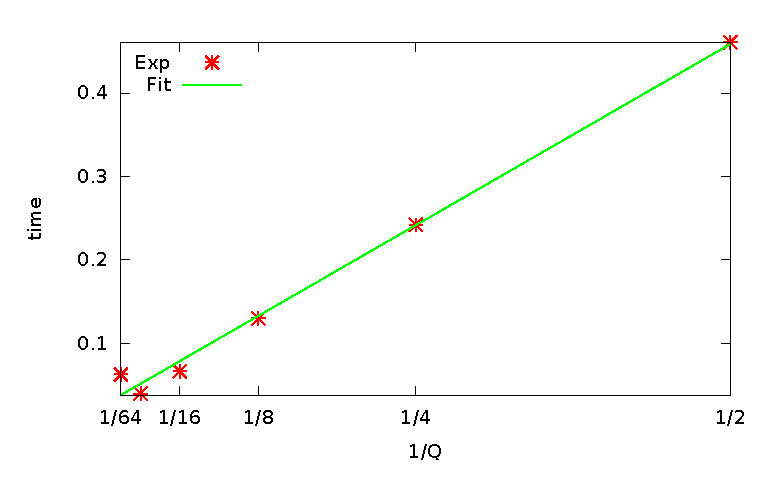
\includegraphics[scale=1.]{t3_exp1.eps}
	\caption{Plot of first set of experiments. The slope is $r M N t_f$, hence $t_f = 8.69$ns.}
	\label{fig1}
\end{figure}

\paragraph{The second set of experiments} we vary $M$ only, and keep $r$, $N$ and $Q$ fixed.  And we can plot a $t_{\textrm{total}} \sim M$ figure.
We also fit this plot by a line. The intercept of this line is $2 r t_s$.  The slope of this line is $r (2 t_w + \frac{N}{Q}t_f)$.
From the intercept and slope, we can get $t_s$ and $t_w$. The setup is that $r=100$, $N=1000$, $Q=32$ and $M=10^3, 2\times10^3, 3\times10^3, 4\times10^3, 5\times10^3$.
The results of the experiments is listed in the Tab \ref{tab3} and is plotted in Fig \ref{fig2} as well. The plot shows very good linearity, and the 
intercept is $3.66\times10^{-3}$, therefore, $t_s = 3.66\times10^{-3}/2/100 = 1.83\times10^{-5}$s. The slope is $3.82\times10^{-5}$, therefore $t_w = (3.82\times10^{-5}/r - \frac{N}{Q}t_f)/2 = 56.5$ns.

\begin{figure}[!htb]
	\centering
	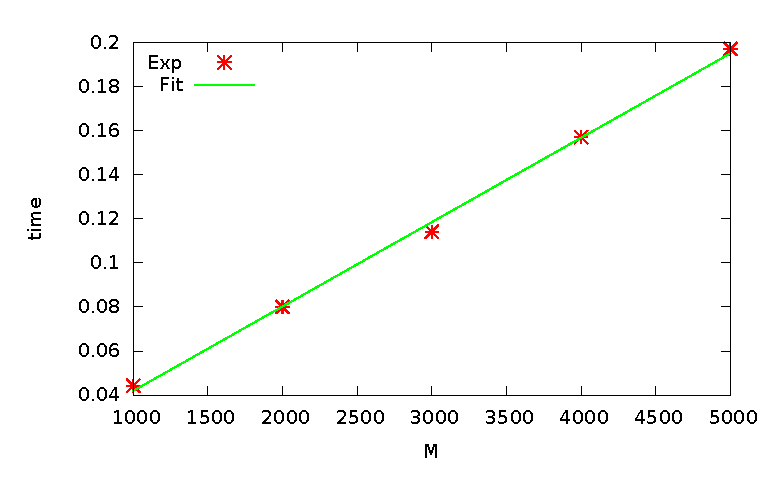
\includegraphics[scale=1.]{t3_exp2.eps}
	\caption{Plot of second set of experiments. The slope is $r (2 t_w + \frac{N}{Q}t_f)$, and intercept is $2 r t_s$ , hence $t_s = 18.3\mu$s, and $t_w=56.5$ns.}
	\label{fig2}
\end{figure}

\begin{table}[h]
	\centering
	\caption{Result of second set of experiments to determine $t_s$ and $t_w$. Varying $M$ and keeping $r, N, Q$ fixed.}
	\label{tab3}
	\begin{tabular}{lllllll}
		\hline
		M                        & $10^3$ & $2\times10^3$ & $3\times10^3$ & $4\times10^3$ & $5\times10^3$ \\ \hline
		$t_{\textrm{total}}$ (s) & $4.42\times 10^{-2}$ & $8.00\times 10^{-2}$ & $1.14\times 10^{-1}$ & $1.57\times 10^{-1}$ & $1.97\times 10^{-1}$ \\ \hline
	\end{tabular}
\end{table}

\subsection{Summary}
So $t_s = 18.3\mu$s, $t_w = 56.5$ns and $t_f = 8.69$ns.

\section{Task 4 The Effect of 2D Process Grids}

\subsection{Implementation}
The case of $P>1$ is similar to that of $P=1$ except the top-bottom communications. 
Since the buffers in the same row is not continuous in memory, it will lead to two different approaches to do top-bottom communication. 
One of them will have a better performance than the other. 
\paragraph{Bad approach } send every element in a row one by one to its neighbors. Therefore, the cost is $(N_loc + 2 w)\cdot (t_s + t_w)$.
This approach is expensive since it will run startup algorithm $N_{loc} + 2w$ times.
\paragraph{Good approach } firstly collect all the element in a row to a continuous buffer, then send that buffer in one time to its neighbors.
The cost is $t_s + (N_loc + 2 w) \cdot t_w$. 

In my implementation, I used the "good approach".

\subsection{Performance Model}
The assumptions made in this model is similar to that in previous section, except that we loose the assumption $P=1$.
We assume that $P>1$ in this section. We also assume $Q$ is larger than $1$. Furthermore, since we use the "good approach",
in each top-bottom communication there will be some overhead due to collecting the elements to a buffer. However, this
overhead is negligible.

The communication cost and computation cost read
\begin{eqnarray*}
	t_{\textrm{comp}} &=& M_{\textrm{loc}} \cdot N_{\textrm{loc}} \cdot t_f \\
	t_{\textrm{comm}} &=& 2 \left[ 2 t_s + \left( N_{\textrm{loc}} + M_{\textrm{loc}} + 2 w \right) \cdot t_w  \right] 
\end{eqnarray*}
$N_{loc} = N/Q$ and $M_{loc}= M/P$. In the left-right communications, only $M_{loc}$ double is sent and received, however, in
the top-bottom communications, $N_{loc} + 2 w$ is communicated. There are four communications per iteration.

Consequently, we can re-write down the performance model 
\begin{eqnarray}
	t_{\textrm{total}} &=& r \cdot \left( t_{\textrm{comp}} + t_{\textrm{comm}} \right) \\
	&=& r \cdot \left[ 4 t_s + 2 \left( \frac{N}{Q} + \frac{M}{P} + 2 w \right) t_w + \frac{M\cdot N}{P\cdot Q} t_f \right] \label{equ2}
\end{eqnarray}

\subsection{Aspect Ratio Effect}
We will analysis Eq \ref{equ2} in this subsection. Notice that $PQ = n$ ($n$ is the number of processes) is fixed, 
$M=N$, the following important relation holds
\[
	\frac{1}{P} + \frac{1}{Q} = \frac{1}{P} + \frac{P}{n} \geq 2 \sqrt{\frac{1}{P}\cdot\frac{P}{n}} = \frac{2}{\sqrt{n}}
\]
the equality holds when $P=Q=\sqrt{n}$.

Taking advantage of above relation, the total cost reads
\begin{eqnarray}
	t_{\textrm{total}} &\geq& r \cdot \left[ 4 t_s + 2 \left( \frac{2M}{\sqrt{P\cdot Q}} + 2 w \right) t_w + \frac{M^2}{P\cdot Q} t_f \right] \label{equ3}
\end{eqnarray}
Consequently, when $P=Q$, the equility holds and the performance is best. As the difference between $P$ and $Q$ increases, the total cost also increases.

\subsection{Experiments}
According to the analysis in above subsection, we set up the experiments as following. The number of processes is chosen to be $nproc = 24$, and we 
do a set of experiments with varying $P = 2, 3, 4, 6, 8, 12$. Other parameters are $M=N=1000, r=100$. The results of the experiments are listed in Tab \ref{tab4}.
The results fit about argument. We can see when $P=6, Q=4$, the cost is lowest among all the cases. It is interesting to see that the case of $P=6, Q=4$ is
different from $P=4, Q=6$. The reason of this phenomena is the top-bottom communications have overhead, such as collecting elements in a row to a temporary buffers.

\begin{table}[h]
	\centering
	\caption{Result of experiments to show the aspect ratio effects. Varying $P$}
	\label{tab4}
	\begin{tabular}{lllllll}
		\hline
		P                        & $2$ & $3$ & $4$ & $6$ & $8$ & $12$ \\ \hline
		$t_{\textrm{total}}$ (s) & $7.41\times 10^{-2}$ & $1.00\times 10^{-1}$ & $7.66\times 10^{-2}$ & $6.27\times 10^{-2}$ & $7.74\times 10^{-2}$ & $6.52\times 10^{-2}$ \\ \hline
	\end{tabular}
\end{table}

\subsection{If $t_f$ is Smaller}
In this model, if $t_f$ is decreased, the overall trends will not change. Since the prefactor of $t_f$ term is a constant for a given number of processes 
and given $M$.

\section{Task 5 Overlapping Communication with Computation}

\subsection{Implementation}
The main part of function \lstinline{parAdvectOverlap(reps, *u, ldu)} is divided into three steps.
\paragraph{First steps} Update the halo by non-blocking sends/receives, and \lstinline{MPI_Wait} will not be used in this part.
\paragraph{Second steps} Update the bulk (inner) field. Bulk is the part of local field which doesn't adjacent to halo. To be more precisely,
its index is $(r,c)$ where $r\in [w+1,N_{loc}+w-2]$ and $c\in [w+1,M_{loc}+w-2]$. Since there is no dependancy on
halo field in updating the bulk field. Therefore, this part of computation can overlap with non-blocking communication.
\paragraph{Third steps} Firstly \lstinline{MPI_Wait} is called in this part. Then making use of the updated halo values,
we can update the boundary field in turn. The boundary is the grids between bulk and halo. To be more precisely,
its index ranges are $(w,w) \sim (w,N_{loc}+w-1)$, $(M_{loc+w-1}, w) \sim (M_{loc+w-1}, N_{loc+w-1})$, 
$(w+1, w) \sim (M_{loc+w-1}, w)$, $(w+1, N_{loc+w-1}) \sim (M_{loc+w-2}, N_{loc+w-1})$. \textit{Attetion}: in
order to update the boundary field, four temporary buffer \lstinline{utmpr}, \lstinline{utmpl}, 
\lstinline{utmpt} and \lstinline{utmpb} are required!
They are used to update right, left, top and bottom boundary, respectively.

\subsection{Performance}
Using non-blocking sends and receives to update halo field firstly,
the program will continue to run the subsequent codes (updating bulk field) which don't depend on halo field values.
Therefore, the communication and computation are overlapping. 

\paragraph{The effets on performance model} The performance model consist three terms, $t_f$ term, $t_w$ term
and $t_s$ term. The last two terms are communication terms. The overlapping approach will decrease $t_w$ term 
significantly by overlapping the communication with computation. However, it will not affect $t_s$ term too much.
Furthermore, if the computation time of the concerned problem is small, the performance will not be improved too much, since the performance is improved by overlapping between computation and communication. We will use it as a guildline to design experiments.

%\paragraph{Experiments} I did two sets of experiments with different $M$ value. The experiment setting is
%$P=1, Q=32$ and $r=100$. The experiment results are shown in Tab \ref{tab5}, which shows overlapping's performance
%is better than the one without overlapping.
%

\paragraph{Experiments} Following the guildline given in previous paragraph, we will vary $N$ and keep $M, r$ and $Q$ fixed. 
The reason of doing so  is in the case of $P=1$, the communication cost only 
depends on $M$ and computation cost depends on both $M$ and $N$. Fixing $M$ and varying $N$ is equivalent to keep communication cost fixed and change the computation cost.
As we argued in previous paragraph, the performance of overlapping method depends on the mount of overlapping between communication and computation. Therefore, we increase $N$ to increase the overlapping part of computation. The experiment settings is $M=1000$, $Q=32$, $P=1$, $r=100$ and $N\in \{10^2, 10^3,10^4, 10^5\}$
We run these experiments with and without overlapping method. The results are shown in Tab \ref{tab5}. Generally, the performance of 
overlapping is better than that without overlapping, except for small $N$. For small $N$ overlapping is a little worse than non-overlapping, since
in my overlapping algorithm, there is some overhead, such as copy values to a temporary field buffers which are used to calculate
boundaries. However, for large $N$, the performance of overlapping is better, and the larger value of $N$, the better performance.
%We also run some additoinal simulation to make the conclusion more solid. These 
%additoinal experiment results are listed in Tab \ref{tab6}. Indeed, overlapping is better.

\begin{table}[h]
	\centering
	\caption{Comparison between overlapping and non-overlapping. Varing $N$}
	\label{tab5}
	\begin{tabular}{lllll}
		\hline
		N               & $10^2$ & $10^3$ & $10^4$ & $10^5$ \\ \hline
		without overlap & $1.08\times10^{-2}$s & $4.13\times10^{-2}$s & $4.24\times10^{-1}$s & $4.19$s  \\ 
		with overlap    & $1.40\times10^{-2}$s & $4.37\times10^{-2}$s & $4.12\times10^{-1}$s & $4.16$s  \\ \hline
	\end{tabular}
\end{table}

%\begin{table}[h]
%	\centering
%	\caption{Comparison between overlapping and non-overlapping. Keeping $M=N$}
%	\label{tab6}
%	\begin{tabular}{lll}
%		\hline
%		                & $M=N=2000$ & $M=N=1000$          \\ \hline
%		without overlap & $0.163$s   & $4.3\times10^{-2}$s  \\ 
%		with overlap    & $0.153$s   & $4.01\times10^{-2}$s \\ \hline
%	\end{tabular}
%\end{table}

\section{Task 6 Wide Halo Transfers}

\subsection{Implementation}
The implementation of wide halo method is quite straightforward. Update the halo with $w$ width every $w$ simulation time steps. 
For each time step in a cycle of total $w$, the part of field to be upated decreases by two.
Therefore, at time step $0$, the size of that part is $(M_{loc}+2*w-2)(N_{loc}+2*w-2)$, at the step $i$, the size is 
$(M_{loc}+2w-2-2i)(N_{loc}+2*w-2-2i)$.
Again, similar to Task 4, in each communication,
we collect $w$ rows/columns into a temporary buffer firstly and then send/receive in one time. This will reduce the $t_s$ term
in communication cost.

\subsection{Performance Model}
There is a trade off in this approach. The startup time $t_s$ part of communication time is decreased by a factor of $w$. However,
the computation cost increases, since one has to do more computation for additional part of field to be updated.

In derivation of the following performance model, we assume that simulation time cycle $r$ is much larger than $w$,
since if it is not, the wide halo method will be worse than the method without wide halo, which is not our interest.
Furthermore, for simplicity, we assume that $r \% w = 0$.

The total time cost is 
\[
	t_{\textrm{total}} = \frac{r}{w} t_{\textrm{cycle}}
\]
where $t_{\textrm{cycle}}= t_{\textrm{comp}} + t_{\textrm{comm}}$ is the cost in one cycle ($w$) of time steps.

For the communication cost per cycle
\[
	t_{\textrm{comm}} = 2 \left[ 2 t_s + w\cdot \left( N_{loc} + M_{loc} + 2 w \right) t_w  \right]
\]

For the computation cost per cycle
\begin{eqnarray*}
	t_{\textrm{comm}} &=& \sum^{w-1}_{0} (M_{loc}+2w-2-2i)(N_{loc}+2*w-2-2i) t_f \\
	&=& w M_{loc} N_{loc} t_f + w(w-1) (M_{loc}+N_{loc}) t_f + \frac{2}{3} w (w-1) (2w-1) t_f
\end{eqnarray*}
where the summation over $i$ reflects the part of field to be updated changes in each time step.

Collecing all the terms, the final total cost is
\begin{equation} \label{equ4}
	t_{\textrm{total}} = r \left[ 
		\frac{4}{w} t_s + 2 \left( M_{loc} + N_{loc} + 2 w \right) t_w +
		M_{loc} N_{loc} t_f + (w-1) (M_{loc}+N_{loc}) t_f + \frac{2}{3}(w-1) (2w-1) t_f
		\right]
\end{equation}
where $N_{loc} = N/Q$ and $M_{loc} = M/Q$.

Comparing wide halo Eq \ref{equ4} with non-wide halo Eq \ref{equ2}, there are two differences.
The first one is the startup term in communication cost decreases by a factor of $w$, since $t_s$ is
a relative large term, so this reduction is not negligible. The second one is the additional computation
cost, which is proportional to $w$ or $w^2$, if $w$ is not small and comparable to $N_loc$ or $M_loc$,
this term is comparable to the non-wide halo computation term $M_{loc} N_{loc} t_f$. Therefore, one 
would be better not to choose a large $w$.

Consequently, in the case where the communication cost is not negligible, the wide halo will have 
a better performance due to the reduction of startup communication $t_s$ term.

\subsection{Experiments}
According to the argument in previous subsection, we should choose the case in which communication cost
is large to do experiments.
Hence we choose $P\neq Q$ and $M\neq N$ from the aspect ratio argument in Task 4. 

In order to investigate the effect of wide halo method, we choose $P=4$, $Q=8$, $N=1\times10^4$, $M=2\times10^4$, 
$r=100$, and vary $w = \{1,5,10,500\}$.  
%In the second set of experiments, we vary $r=\{1,10,10^2,10^3\}$ and keep $w=5$. 
I choose a large $w$ to show that when $w$ is large the total cost will increase due to the additional computation cost.
The results are shown in Tab \ref{tab7}. The case of $w=1$ is the one without wide halo effect, we can 
see that when $w$ increases (except the case $w=500$), the total time decreases, so the wide halo method is effective. 
Furthermore, when $w=500$, the total cost increases by almost a factor of $2$. This is because when $w=500$, which
is near $N_{loc} = 10^4/8 = 1250$, the additoinal computation cost is comparable to the original one.

\begin{table}[h]
	\centering
	\caption{Wide halo effect. Experiment Set 1, varying $w$ and keep $r, P, Q, M, N$ fixed.}
	\label{tab7}
	\begin{tabular}{lllll}
		\hline
		w               & $1$ & $5$ & $10$ & $500$ \\ \hline
		time            & $8.65$s & $8.52$s & $8.21$s & $16.7$s  \\ \hline
	\end{tabular}
\end{table}

\subsection{Comparison with Overlapping Method}
The wide halo method will reduce the startup communication cost, the $t_s$ term.  
The overlapping method will also reduce the communication cost, however, it reduce the 
data transfering term, the $t_w$ term, by overlapping it with computation.

Consequently, both methods will reduce the communication cost, but from different aspects.

\section{Task 7 Literature Rewiew on Cache Oblivious}

In following paragraphs, we will first introduce cache oblivious algorithm,
and then discuss its application and impacts in stencil computation.

\vspace{\baselineskip}

Reduction of cache miss is one of important aspect of algorithm optimization.
It is also true in parallel computation, which highly emphasizes on the performance of algorithm.
Many programmers is aware of this fact and implement their algorithm with the consideration of cache miss.
However, many of such algorithms will depend on the parameters of cache, such as cache line size and the number of cache line.
These cache parameters are actually relevant to hardware, which is out of control of programmer.
Consequently, one program optimized with some specific cache parameter may have very low performance on a machine with another set of cache parameters. 
Furthermore, in modern computers, there are more than one level of caches with difference cache parameters, which make the above issues more serious.
To solve this problem, Frigo and his collabrators \cite{Frigo1999} proposed the idea of cache oblivious algorithm for tall cache in parallel programming. 
Their cache oblivious algorithm doesn't know the cache parameters, 
but uses caches as effeciently as those algorithms who knows cache parameter foreahead.

In the master thesis of Prokop \cite{Prokop1999} applied the cache oblivious method to stencil problem for the first time.
But his algorithm can only work for one dimension space problem with square spacetime region.
In 2005, Frigo proposed an algorithm which can work for arbitrary stencil and arbitrary spacetime dimension \cite{Frigo2005}.
In this paper, the spacetime concerned in the problem is divided into \textit{trapezoidal regions}.
If the flow velocity is zero, the the trapezodial regions become rectangular regions.
Once the the field value $u$ at the bottom edge(or surface or cube, depending on the space dimension) of the trapezodial region is known, 
the whole $u$ values in the trapezodial region can be obtained by applying the approciate fluid equations.
These trapezodial regions can be divided into smaller trapezodial region with nearly equal size.
This dividing process can be done iteratively until each trapezodial region is small enough to entirely fit in cache.
Therefore, in this method, the field values are not calculated in the order of their spatial index any longer, 
but in the order of trapezodial region index.
Frigo proofs this method is cache efficient \cite{Frigo2005}.

Making use of this method, cache miss is reduced. For example, Frigo \cite{Frigo2007} applied this method to heat diffusion problem.
For two dimension problem, the cache miss will be reduced by a factor of 5 on average, 
and for one dimension heat diffusion problem, the cache miss will be reduced to $1\%$ \cite{Frigo2007},
Therefore, the cache oblivious method improves the performance of parallel stencil problem by reducing the cache miss.




\section{Task 8 Optional}

I choose to implement overlapping code for $P>1$ as an optional task.

\vspace{\baselineskip}

The idea of the solutioin to this problem is similar to the case for $P=1$ in task 5.
But in this case, the main part of \lstinline{parAdvectExtra} contains five parts. 
\paragraph{First part} Non-blocking communication the left and right halo. Don't do \lstinline{MPI_Wait} in this step.
\paragraph{Second part} Update the field values in the bulk. The definition of bulk is the same as that for $P=1$ in task 5.
\paragraph{Third part} \lstinline{MPI_Wait} for left and right halo communication here.
\paragraph{Fourth part} Top and bottom communications. I implement in non-blocking communication but \lstinline{MPI_Wait} immediately. Therefore, it is essential a blocking communication.
\paragraph{Fifthe part} Update the field value on the boundary. The definition of boundary is the same as that for $P=1$ in task 5. Also use four temporary buffers.

\vspace{\baselineskip}

I run two experiments with parameters $P=4$, $Q=2$, $M=N=1000$, $r=100$ with and without \lstinline{-x} option. 
The one with overlapping method uses time $0.152$s, and the one without overlapping method uses $0.154$s.


\section{Deficiencies}
I should make the code more robust. For example, $w$ should be smaller than $N_{loc}$
and $M_{loc}$ mathematically. I should add some code to tell the user if they 
input the wrong parameters.

In task 4 ratio aspect effect, from model, the larger difference in $M$ and $N$,
the more total cost. However, my results has some fluctuations.

In task 5 overlapping, I use temporary buffer $utmpt$, $utmpb$, $utmpl$ and $utmpr$
to update the field values on boundaries so that we can decouple the bulk calculation
with the field values on the halo. The trade off of this approach is that we have to
copy values to this four buffers, which generates some overhead. So in some situation,
the overlapping method will be a little worse than  the non-overlapping one, although
their different is very small.

In task 8 overlapping for $P>1$, there are 4 communications in each iteration. But
only first two of them is overlapped with computation. The last two communications
don't overlap with computation. This is a deficiecy.

\section{Feedback}
In the experiments results, there is always some "fluctuations", I can't understand
what's the reason of these fluctuations, so I think it is better to know some details
on message communication, such as what's factor will affect $t_s$ and so on.





%%%%%%%%%%%%%%%%%%%%%%%%%%%%%%%%%%%%%%%%%%%%%%%%%%%%%%%%%%%%%%%%%%%%%%%
%%%%%%%%%%%%%%%%%%%%%%%%%%%%%%%%%%%%%%%%%%%%%%%%%%%%%%%%%%%%%%%%%%%%%%%

\acknowledgments
Thanks Peter for nice lectures, Sara for her lab tutorial and  Raijin for providing the computing resource.
\appendix

%\section{Appendix I}

%\begin{thebibliography}{999}
%\end{thebibliography}
\bibliography{citation}
\bibliographystyle{plain}
\end{document}
